\input ../talk-header.tex
\title{Machine Learning}
\subtitle{Random Forests}

% If you wish to uncover everything in a step-wise fashion, uncomment
% the following command: 
%\beamerdefaultoverlayspecification{<+->}

\begin{document}

\begin{frame}
  \titlepage
\end{frame}


\begin{frame}
  \frametitle{Decision Trees}
  \only<1>{
    % https://www.pexels.com/photo/blue-geeen-and-orange-parrot-37833/
    % https://static.pexels.com/photos/37833/rainbow-lorikeet-parrots-australia-rainbow-37833.jpeg
    % CC0 license
    \vspace{-2cm}
    \cimgwb{rainbow-lorikeet-parrots-australia-rainbow.jpg}
  }
  \only<2>{\centerline{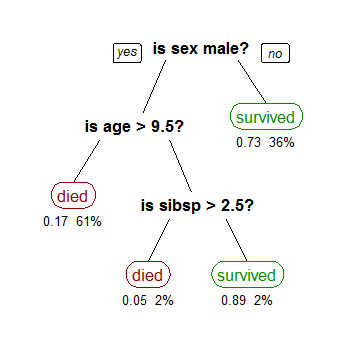
\includegraphics[height=.9\textheight]{tree_titanic_survivors.png}}
    % https://commons.wikimedia.org/wiki/File:CART_tree_titanic_survivors.png
    % License: CC ASA 3.0 unported.

    \vspace{-28mm}\parbox{.4\textwidth}{\red{E.g., passengers died
        with probability .17 which is 61\% of observations}}

    %\vspace{-18mm}
    \prevwork{Stephen Milborrow}
  }
  \only<3>{
    Variations
    \begin{itemize}
    \item Classification tree
    \item Regression tree
    \end{itemize}
  }
  \only<4>{
    % https://www.pexels.com/photo/nature-bird-australia-owl-105810/
    % https://static.pexels.com/photos/105810/pexels-photo-105810.jpeg
    % CC0 license
    \vspace{-3cm}
    \cimgwb{owl.jpg}
    \vspace{-8.7cm}
    \phrase{What can go wrong?}
  }
  \only<5>{
    Ensemble methods
    \begin{itemize}
    \item Bagging
    \item Random forest
    \item \gray{Boosted trees \textit{ (gradient boosted trees)}}
    \item \gray{Rotation forest}
    \end{itemize}
  }
\end{frame}

\begin{frame}
  \frametitle{Boostrap aggregating = bagging}
  \only<1>{\phrase{Boostrap}

    A family of statistical methods using sampling with replacement.
  }
  \only<2>{
    \begin{itemize}
    \item Increase stability
    \item Increase accuracy
    \item Reduce variance
    \item Avoid overfitting
    \end{itemize}
    A type of model averaging.
  }
  \only<3-4>{
    \begin{itemize}
    \item Training set $D$ of size $n$
    \item Sample $D$ \textit{with replacement} to create $D_1, \ldots, D_k$ of size $n'$
    \item If $n=n'$, expect $1-1/e \approx 63.2\%$ repeats
    \end{itemize}
  }
  \only<4>{
    \begin{itemize}
    \item Train $k$ models
    \item Average (regression) or vote (classification)
    \end{itemize}
  }
  \only<5>{
    Do not confuse with
    \begin{itemize}
    \item Boosting (and AdaBoost)
    \item Boostrap (statistics)
    \item Cross validation
    \end{itemize}
  }
\end{frame}

\begin{frame}
  \frametitle{Random subspace method}
  \only<1>{
    \phrase{attribute bagging = feature bagging}
  }
  \only<2>{
    \blue{Bagging (bootstrap aggregation)} = resampling to create more
    data sets, train models on different samples

    \blue{Attribute bagging} = project to create more data sets, train
    models on different samples
  }
\end{frame}

\begin{frame}
  \frametitle{Random forests}
  \only<1>{
    \vspace{1cm}
    \centerline{Combine \blue{bagging} with \blue{random subspace method}}
  }
\end{frame}

%%%%%%%%%%%%%%%%%%%%%%%%%%%%%%%%%%%%%%%%%%%%%%%%%%%%%%%%%%%%%%%%%%%%%%
%\talksection{Break}

\begin{frame}
  % https://www.pexels.com/photo/branches-fog-forest-landscape-235635/
  % https://static.pexels.com/photos/235635/pexels-photo-235635.jpeg
  % CC0 license
  \cimgwb{forest.jpg}
  \vspace{-9cm}
  \phrase{questions?}
\end{frame}

\end{document}
